%%%%%%%%%%%%%%%%%%%%%%%%%%%%%%%%%%%%%%%%%%%%%%
% Head matter - can we try to be consistent on
% included packages
\ifdefined\beamerclass
\else
    \def\beamerclass{beamer}
\fi
\documentclass[\beamerclass]{beamer}

\usepackage{pgfpages}
\mode<handout>{
  % \setbeamercolor{background canvas}{bg=black!20}
  \pgfpagesuselayout{2 on 1}[a4paper,border shrink=5mm]
}

%\documentclass{beamer}
\mode<presentation>
{\usetheme{default}
 \usecolortheme{default}
 \usefonttheme{default}
 \setbeamertemplate{navigation symbols}{}
 \setbeamertemplate{footline}[frame number]
% \setbeamertemplate{caption}[numbered]
 }
\usepackage[english]{babel}
\usepackage{algorithm}
\usepackage[noend]{algpseudocode}
\usepackage[utf8x]{inputenc}
\usepackage{graphicx}
\usepackage{hyperref}
%\graphicspath{{./images/}}
\usepackage{tikz}
\usetikzlibrary{shapes.geometric, arrows,chains}
\usepackage{booktabs,makecell,multirow,tabularx}
\usepackage{verbatim}
\renewcommand{\arraystretch}{1.2}
\renewcommand\theadfont{\normalfont\bfseries}
\usepackage{array}
\usepackage{listings}
\lstset{language=Java, showstringspaces=false}
\usepackage[normalem]{ulem}
\usepackage{bm}
\def\layersep{2.5cm}

\usepackage{xcolor}
%\usepackage{subfig}
\setbeamertemplate{caption}{\insertcaption}
\usepackage[caption=false]{subfig}
\usepackage{hyperref}
\usepackage{verbatim}
%\setbeamertemplate{caption}[numbered]%\numberwithin{figure}{section}
% Define block styles

\usetheme{Copenhagen}
\hypersetup{pdfstartview={Fit}}
\lstset{basicstyle=\small\ttfamily,breaklines=true}

\usepackage{xmpmulti}

\tikzstyle{decision} = [diamond, draw, fill=blue!20, 
    text width=4.5em, text badly centered, node distance=3cm, inner sep=0pt]
\tikzstyle{block} = [rectangle, draw, fill=blue!20, 
    text width=3em, text centered, rounded corners, minimum height=3em]
\tikzstyle{line} = [draw, -latex']
\tikzstyle{cloud} = [draw, ellipse, fill=red!20, node distance=3cm,
    minimum height=2em]
\tikzset{
  startstop/.style={
    rectangle, 
    rounded corners,
    minimum width=3cm, 
    minimum height=1cm,
    align=center, 
    draw=black, 
    fill=red!30
    },
  process/.style={
    rectangle, 
    minimum width=3cm, 
    minimum height=1cm, 
    align=center, 
    draw=black, 
    fill=blue!30
    },
  decision/.style={
    rectangle, 
    minimum width=3cm, 
    minimum height=1cm, align=center, 
    draw=black, 
    fill=green!30
    },
  arrow/.style={thick,->,>=stealth},
  dec/.style={
    ellipse, 
    align=center, 
    draw=black, 
    fill=green!30
    },
}
\tikzstyle{arrow} = [thick,->,>=stealth]

\tikzset{onslide/.code args={<#1>#2}{%
  \only<#1>{\pgfkeysalso{#2}} % \pgfkeysalso doesn't change the path
}}

\makeatletter
\newenvironment<>{btHighlight}[1][]
{\begin{onlyenv}#2\begingroup\tikzset{bt@Highlight@par/.style={#1}}\begin{lrbox}{\@tempboxa}}
{\end{lrbox}\bt@HL@box[bt@Highlight@par]{\@tempboxa}\endgroup\end{onlyenv}}

\newcommand<>\btHL[1][]{%
  \only#2{\begin{btHighlight}[#1]\bgroup\aftergroup\bt@HL@endenv}%
}
\def\bt@HL@endenv{%
  \end{btHighlight}%   
  \egroup
}
\newcommand{\bt@HL@box}[2][]{%
  \tikz[#1]{%
    \pgfpathrectangle{\pgfpoint{1pt}{0pt}}{\pgfpoint{\wd #2}{\ht #2}}%
    \pgfusepath{use as bounding box}%
    \node[anchor=base west, fill=orange!30,outer sep=0pt,inner xsep=1pt, inner ysep=0pt, rounded corners=3pt, minimum height=\ht\strutbox+1pt,#1]{\raisebox{1pt}{\strut}\strut\usebox{#2}};
  }%
}
\makeatother

\definecolor{darkblue}{RGB}{37,55,97}
\definecolor{mellowyellow}{RGB}{247,206,70}
\definecolor{almostwhite}{RGB}{254,255,255}
\definecolor{merrygreen}{RGB}{79,173,91}
\definecolor{funkyorange}{RGB}{240,154,56}

\addtobeamertemplate{footnote}{\hskip -2em}{}
\newcommand\blfootnote[1]{%
  \begingroup
  \renewcommand\thefootnote{}\footnote{#1}%
  \addtocounter{footnote}{-1}%
  \endgroup
}

\DeclareMathOperator{\softmax}{softmax}
\DeclareMathOperator{\ReLU}{ReLU}

%%%%%%%%%%%%%%%%%%%%%%%%%%%%%%%%%%%%%%%%%%%%%%
% Formatting for title page
\title[Auto-encoders]{Unsupervised and self-supervised learning}
\subtitle{Auto-Encoders}
\author{Jonathon Hare}
\institute[]
{
  Vision, Learning and Control\\
  University of Southampton 
}
\date{}
\subject{Computer Science}
\useoutertheme{infolines}
\setbeamertemplate{headline}{} %remove headline
\setbeamertemplate{navigation symbols}{} %remove navigation symbols
%%%%%%%%%%%%%%%%%%%%%%%%%%%%%%%%%%%%%%%%%%%%%%

\begin{document}

\begin{frame}[plain]
        \begin{tikzpicture}[overlay, remember picture, shift={(current page.south west)},font={\fontfamily{Montserrat-TOsF}\selectfont}]
        \fill [mellowyellow,text=almostwhite] (0,0) rectangle (\paperwidth, \paperheight);
        \draw (5.5,7) node [align=left,text=darkblue] {\Huge 
        \begin{tabular}{l} 
        \textbf{Learn}\\
        \textbf{Latent} \\
        \textbf{Representations} 
        \end{tabular}};
        \draw (11,1) node [align=left,text=darkblue] {\includegraphics[scale=0.15]{../vlc.png}};
        \end{tikzpicture}
\end{frame}

\begin{frame}
  \titlepage
\end{frame}
%-------------------------------------------------------------%
\begin{frame}
\frametitle{Compressed and Latent Representations}

\end{frame}

\begin{frame}
\frametitle{Compression}

\end{frame}

\begin{frame}
\frametitle{Generative Modelling from Latent Representations}

\end{frame}

%-------------------------------------------------------------%
\begin{frame}
\frametitle{Autoencoders}
The aim of an autoencoder is to learn a representation (encoding) for a set of data, typically for dimensionality reduction, by training the network to ignore signal noise. 
\begin{center}
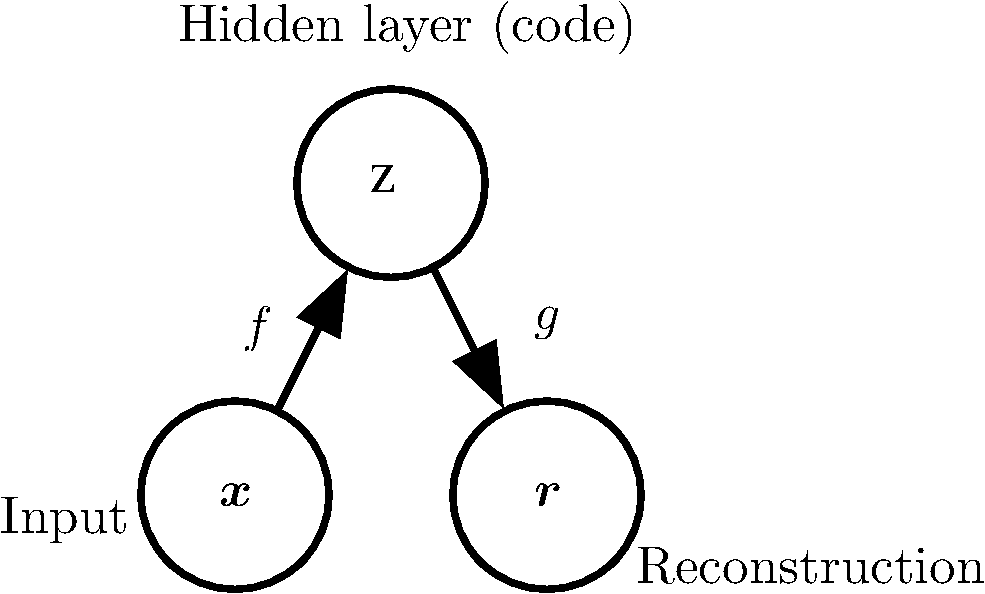
\includegraphics[width=7cm]{AE.pdf}
\end{center}
\end{frame}
%-------------------------------------------------------------%

\begin{frame}[fragile]{pause}\frametitle{Deep Autoencoders}
\begin{center}
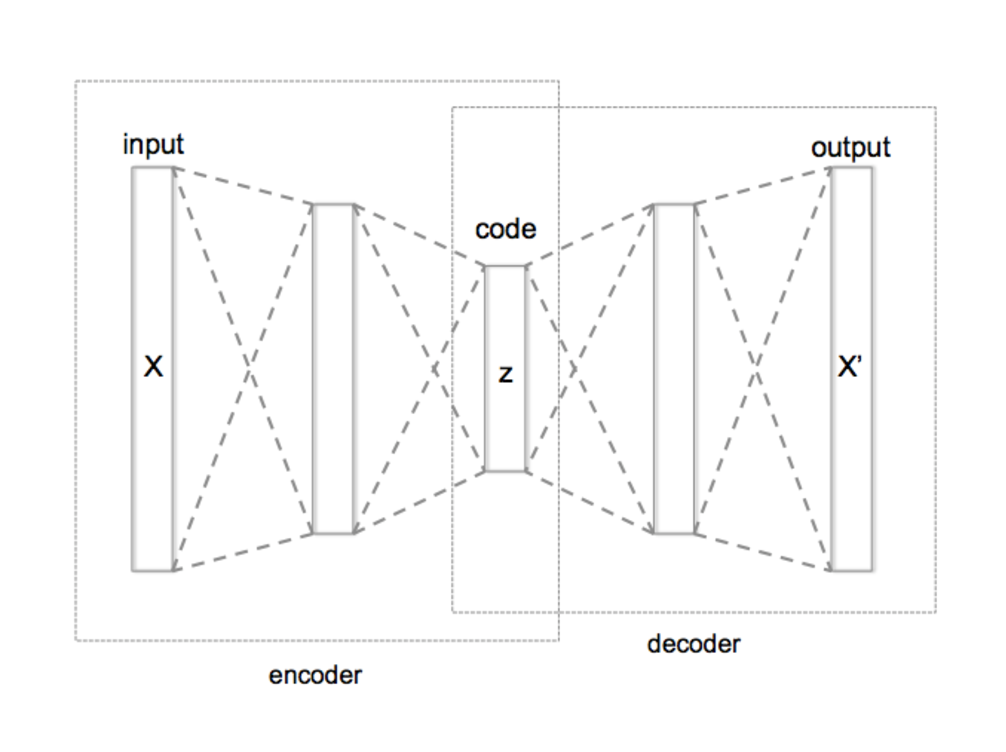
\includegraphics[width=10cm]{DAE.pdf} \footnote{Image taken from wikipedia}
\end{center}
\end{frame}
%-------------------------------------------------------------%

\begin{frame}
\frametitle{Denoising Autoencoders}

\begin{itemize}
\item<+-> Denoising autoencoders take a partially corrupted input and train to recover the original undistorted input.
\item<+-> To train an autoencoder to denoise data, it is necessary to perform a preliminary stochastic mapping to corrupt the data ($x \rightarrow \tilde x$). 
\item<+-> A normal autoencoder is used with $\tilde x$ is used as input and $ x$ as output.
\item<+-> In a denoising autoencoder, the loss should be computed on $\mathcal{L}(x, \hat x)$ as opposed to $\mathcal{L}(\tilde x, \hat x)$.
\end{itemize}
\end{frame}
%-------------------------------------------------------------%
\begin{frame}[fragile]{pause}\frametitle{Sparse Autoencoders}
\begin{itemize}
\item In a sparse autoencoder, there are more hidden units than inputs, but only a small number of the hidden units are allowed to be active at the same time.
\end{itemize}
\end{frame}
%-------------------------------------------------------------%
\begin{frame}
\frametitle{Convolutional Autoencoders}
\begin{itemize}
\item 
\end{itemize}
\end{frame}
%-------------------------------------------------------------%

\begin{frame}\frametitle{Autoencoder Applications}
\begin{itemize}
\item<+-> Any basic AE (or its variant) is used to learn a compact representation of data.
\item<+-> You can learn automatic features from data.
\item<+-> Denoising can help generalise over the test set since the data is distorted by adding noise.
\item<+-> Pretraining networks by learning your network weights using a stacked AE.
\end{itemize}
\end{frame}

\end{document}